%  Written for Columbia COMS4115, fall 2008
\documentclass[onecolumn,titlepage]{article}
\usepackage[pdftex]{graphicx}
\usepackage{fullpage}
\usepackage{moreverb}
\usepackage{multicol}
\usepackage{hyperref}
\usepackage{setspace}
\usepackage{listings}

\hypersetup{
    bookmarks=true,         % show bookmarks bar?
    unicode=false,          % non-Latin characters in Acrobat’s bookmarks
    pdftoolbar=true,        % show Acrobat’s toolbar?
    pdfmenubar=true,        % show Acrobat’s menu?
    pdffitwindow=true,      % page fit to window when opened
    pdfborder={0 0 0},
    pdftitle={CuLOG},    % title
    pdfnewwindow=false,      % links in new window
    colorlinks=true,       % false: boxed links; true: colored links
    linkcolor=black,          % color of internal links
    citecolor=black,        % color of links to bibliography
    filecolor=blue,      % color of file links
    urlcolor=blue           % color of external links
}

\lstset{numbers=left, numberstyle=\small, stepnumber=1}
\lstset{commentstyle=\textit, captionpos=tb, frame=TB}

\onehalfspace


\def\sourcetabsize{4}
\newenvironment{sourcestyle}{\begin{scriptsize}}{\end{scriptsize}}
\def\sourceinput#1{\par\begin{sourcestyle}\verbatimtabinput[\sourcetabsize]{#1}\end{sourcestyle}\par}

\usepackage{float}
 
\floatstyle{ruled}
\newfloat{program}{thp}{lop}
\floatname{program}{Program}


\begin{document}
\title{C$\mu$LOG Project Final Report\\\small{An Entity Interaction Simulation Language}}
\author{John Demme (jdd2127)\\Nishant Shah (nrs2127)\\Devesh Dedhia (ddd2121)\\Cheng Cheng (cc2999)
\\ \\Columbia University}

\maketitle

\tableofcontents

\section{Introduction: C$\mu$LOG}

C$\mu$LOG is a logic language designed for entity interaction
simulation. It uses a brute force method for solution searching similar
to Prolog but uses a syntax similar to C, making it easier on the
typical programmer's eyes, and is compatible with some code
tools, such as code indenters and Emacs's c-mode.

Simulations in
C$\mu$LOG involve a set of entities written in C$\mu$LOG which
interact in the simulator.  The ``environment'' entity defines the
board on which the ``agents'' play, and defines the game which the
entities play.  It is a turn-based simulation during which each agent
can look at the contents of the environment and decide which which
direction it should move.  During this decision, the agents can modify
their own working memory, thus affecting their decision for the next
turn.

Additionally, the C$\mu$LOG interpreter may be invoked separately from
the simulator.  The stand-alone interpreter searches for all the
solutions for ``main'', but typically the output of these programs
will be from ``print'' directives specified in the program.

\subsection{Application \& Features}

One uses the language to provide a set of facts and rules, and the
program is run by asking a question, which the interpreter attempts
to answer using inferences based on the fact and rule set. C$\mu$LOG is
designed for simulation, so typically a simulator will ask a given
agent program what it’s next action will be. The agent program then
uses C$\mu$LOG's entity interaction features to gather information about
it’s environment and decide what to do. Each agent program can
communicate with other programs to find out more information about
other agents or its own status in the environment. The simulator stores
all the contextual information pertaining to the environment and all
of the agents present.

As this language is going to be used for simulating real life agents,
we strongly emphasize that the program learn and forget
data/rules/information at run-time. For this, similar to ``assert'' and
``retract'' of Prolog we have introduced two directives called ``learn''
and ``forget.'' In C$\mu$LOG there exist no specific data structures like
you would see in Java or Python, however rules and facts can be added
to the program dynamically, which allows programs to remember data in
a much more natural way since the data simply becomes part of the
running code. 

The simulator discussed could be modified to be used in other
with other simulation environments, such as in a three-dimensional grid
simulation with several agents--such as a flight simulation. Alternatively,
the interpreter could be used in a real environment like the movement
of pick and
place robots in a warehouse. The language could be used to define the
warehouse environment and agent programs for robots, and a replacement
for the simulator would feed live information in to the programs in
the form of facts, similarly to how the simulation feeds its state
information to agents now.

\subsection{Goals}

The language and simulator presented here attempts to fulfill the
following requirements:
\begin{description}
  \item[Generic] Games are defined mostly by the environment
    application.
    
  \item[Composable] Individual behaviors can be written simply and
    easily, then combined to obtain high-level actions and reasoning
    
  \item[Declarative] Programmers can specify what they want
    entities to do rather than how

  \item[Controlled Communication] Data in the system is frequently
    made up of nearly-atomic bits of data many of which can be used
    both on their own and composed as complex data. This means that
    subsets and smaller pieces of data can be communicated between
    entities without loosing meaning.

  \item[High-level libraries] Due to the flexibility and composibility
    of the language, high-level
    algorithms–-such as path finding–-can be easily implemented in
    libraries, allowing further, domain-specific intelligence to be
    written in the programs.
\end{description}

\section{Tutorial}

Logic programming is a kind of computer programming using mathematical
logic. Specifically, it is based on the the idea of applying a
theorem-prover to declarative sentences and deriving
implications. Compared with procedural languages, logic programming
solves the problem by setting rules with which solutions must fit. We
can represent logic programming by the formula:

$Facts + Rules = Solutions$

Logic programming languages are inherently high level
languages, allowing programmers to specify problems in a declarative
manner, leaving some or all of the details of solving the problem to
the interpreter. 

Both the programming and data
structures in both prolog and C$\mu$LOG can be very simple- such as
facts. The relationship between code and data is also of note. C$\mu$LOG
uses the Von Neumann style (vs. Harvard architecture) wherein data is
code. It is therefore possible (and inherently necessary) for programs
to be introspective and self-modifying. In other words, it is easier
for programs to learn and adapt.


\subsection{Variables}
Variables represent a value to be solved for. They don't have a fixed
datatype, but match to the refered type. All variables are scoped to
the rule, so that variable solutions can be shared between sub-blocks.

Variables are represented by a dollar sign (\$) then the variable
name. The name must start with a letter, and is composed of letters,
numbers, and underscores. There is a special variable called the
anonymous variable which is represented simply by a question mark (?).


\begin{verbatim}
Example variable names:
   $foo  $bar_  $f1o2o3
\end{verbatim}

\begin{verbatim}
The following are not valid variables:
  foo  $_foo  $1bar
\end{verbatim}

\subsection{Statements}

These are conditional statements which give output as true or false
only and are frequently used to constrain variables. They are of two
types, comparison and evaluation statements.

Comparison statements are used to compare variables against constants:

\begin{verbatim}
Example comparisons:
  $a>1+3-4; //means that variable 'a' is always greater than 0
  $boo <= 5; // means that variable 'boo' is less than or equal to 5
\end{verbatim}

Evaluation or eval statements are used to query the program for solutions:

\begin{verbatim}
  boofar($s,$d,7); //from all the possible matches in the program's
     //graph it returns various possible values for the pair s and d,
     //and constrains those values in their scope appropriately, as 
     //defined by the block in which the statement is contained
\end{verbatim}

\subsection{Facts}

Facts are terminal nodes of the solution search which are always
true. Facts help us define constant information in the program like
the position of a wall.

\begin{verbatim}
Syntax: id(parameter1, parameter2 ....);

Examples:
  wall(2,3);  //This means that a wall is defined for 2 and 3

  fire(4,a); //Symbols like 'a' can also be a parameter.
             // Here, fire of 4 and 'a' evaluates to be true.
\end{verbatim}


\subsection{Rules}
Rules are similar to facts, but are only conditionally true. These
conditions are defined inside a block. The defination or declaration
of rules suggests that the solution tree is about to branch out to
search for new solutions.


\begin{verbatim}
  syntax: id(parameter1, parameter2....) {conditions}
\end{verbatim}

The block is "{conditions}" in the above syntax. Block can be of 2
types, namely 'AND' and 'OR' block. AND blocks evalute true iff all
the conditions inside the block are true. Similarly, the OR block is
true if any one of the conditions is true. If no reduction method is
specified (i.e. AND or OR is written), by default AND is used.

To define a OR block we use the following construct:

\begin{verbatim}
  {OR:
    foo();
    bar();
  }
\end{verbatim}

The AND block is written similarly:

\begin{verbatim}
  wall(2,3) {AND:
    foo();
    bar();
    {OR: barfoo(); foobar();}
  }
\end{verbatim}

Here ``{OR: barfoo(); foobar();}'' is a sub-block. wall(2,3) is
true if foo() and bar() are true and if either of barfoo() or foobar()
are true.

\subsection{Directives}
Three interpreter directives are supported; print, learn and
forget. print is used to output strings and results during
runtime. the learn and forget directives are used for database
modification. They function similar to assert and retract of prolog.

\begin{verbatim}
Syntax: @directive_name(parameters);

Example:
     //prints "hello world: " then whatever constraints exist on $foo
  @print("hello world:", $foo);

    //adds a fact to the database that 'fire' is true for 4,5
  @learn(fire(4,5););

    //erases the fact from the database that tree is true for 3,9.
  @forget(tree(3,9););
\end{verbatim}

\subsection{Simulator}

Now for the user to be able to run a simulation or play a game in
C$\mu$LOG, they will have to use a simulator which interacts with the
logic engine of the langauge to produce required results. For
demonstration we have done so already. This simulator defines a class
of games or simulations described as follows:

The environment is grid based and defined by a C$\mu$LOG program. It
potentially includes obstacles and a goals which the agent must reach,
however the game is defined mostly by the environment
program. Every object (i.e. agents, walls, switches, goals) in the
environment is defined by grid positions. The environment specifies
the representations of the entities to the simulator. The simulator
re-evaluates the various object rules during each turn when it renders the
grid, so the contents of the grid can be dynamically defined based on
the state of the simulation or the contents of the program (which can
be changed by the program.) For example based on the grid position of
the agent the environment might remove or insert a wall. The agent
program decides the next move based on previous moves and obstacle
data.

The simulation of the agent program is also turn based. Each time the
agent makes a move it sends its new coordinates to the simulator. The
new coordinates become part of the simulation's state which are
exposed to the environment when it is solved to render the scene.

\begin{verbatim}
Example 1:
  Size(5,5);  //defines the grid size of 5 by 5
  wall(2,3);  //a fact where wall is present at coordinates 2,3 	
  wall(4,2);
  goal(3,3);  //a fact which defines the goal to be achieved by the player	

  igo("UP");  //move($dir) would be true for all the values of $dir
              // for which igo($dir) is true

  move($dir){
        //causes the interpreter to remove igo("UP") from its database.
    @forget(igo($dir);); 

        //Fetch the next movement 
    igo($dir);
  }

The output of the above program is:
X

. . . . .
. . . . .
. | # . .
x . . | .
. . . . .
\end{verbatim}


In the above example, 'size', 'goal', 'wall' and 'move' are keywords
for the simulator.  Size(5,5) defines the grid in which walls (shown by
the pipe symbol) are placed at coordinates (2,3) and (4,2). A goal
object (shown by \#) is placed at (3,3).  The game simulation ends when
the agent either hits a wall, moves out of the grid or reaches the
goal. 

In order to run code through the simulator, put your code in a file
with a ``.ul'' extension (this extension is a convention only) then
invoke the simulator, passing it the name of your code file:

\begin{verbatim}
  ./simulator mySimulation.ul
\end{verbatim}

\subsection{Program Modification}

Now let us look at example using one of our program modification
directives.

\begin{verbatim}
Example 2:
  size(5, 5);
  wall(2, 3);
  wall(4,2);
  goal(3, 3);
  imove("UP");
  imove("RIGHT");
  imove("RIGHT");
  imove("UP");

  move($dir) {
    @forget1( imove($dir); );
    imove($dir);        
  }

OUTPUT:

  ==== Turn 1 ====
  . . . . .
  . . . . .
  . | # . .
  x . . | .
  . . . . .

  x: Moving RIGHT

  ==== Turn 2 ====
  . . . . .
  . . . . .
  . | # . .
  . x . | .
  . . . . .

  x: Moving RIGHT

  ==== Turn 3 ====
  . . . . .
  . . . . .
  . | # . .
  . . x | .
  . . . . .

  x: Moving UP

  Simulation over: x wins!!!Successfully reach the goal at position (3,3)
\end{verbatim}

In the above code we see a carefully drafted route through the
grid can make you win the game. Each step of the simulation is
displayed. In this example, the 'imove' facts are used as a stack of
moves which are queried for each turn, and removed from the stack
after using it.  The ``@forget1'' directive shown in this example
removes only one fact from the program instead of all the facts which
match the pattern.

\subsection{Breakout}

Although we can define an agent's actions within the environment
program, it is typically more desirable to specify a separate agent
file so that multiple agents can operate in the same environment.  In
the next example, we use a separate agent which queries the
environment for the movements it should take--sort of like asking for
directions.

\begin{verbatim}
Environment Program:
  size(10, 10);
  wall(?, 7);
  goal(6, 6);

  imove("UP");
  imove("RIGHT");
  imove("RIGHT");
  imove("RIGHT");
  imove("RIGHT");
  imove("RIGHT");

  agent("d", "tests/agents/delg_to_env.ul");

Agent Program:
  move($dir) {
    @print($e, " says move ", $dir);
    $e.@forget( imove($dir) );
    env($e);
    $e.imove($dir);
  }
\end{verbatim}


\section{Language Reference Manual}

\subsection{Lexical}
\begin{verbatim}
[' ' '\t' '\r' '\n'] WS
"/*"     OPENCOMMENT
"*/"     CLOSECOMMENT
"//"     COMMENT
'('      LPAREN
')'      RPAREN
'{'      LBRACE
'}'      RBRACE
';'      SEMICOLON
','      COMMA
'+'      PLUS
'-'      MINUS
'*'      TIMES
'/'      DIVIDE
"=="     EQ
'<'      LT
"<="     LEQ
">"      GT
">="     GEQ
'@'      AT
'.'	 DOT
'"'      QUOTE
'?'      QUESTION
'!'      NOT
'$'['a'-'z' 'A'-'Z']['a'-'z' 'A'-'Z' '0'-'9' '_']* Variable
['0'-'9']+ Number
['a'-'z' 'A'-'Z']['a'-'z' 'A'-'Z' '0'-'9' '_']* Identifier
\end{verbatim}

\subsection{Facts}
Facts define factual relationships.  They have a very similar syntax to rules, except they
have no code block to make them conditionally true.  Any query which matches a fact is simply
true. Another way to think of facts is as terminal nodes in the solution search.

Each fact is composed of a name, and a comma separated list of parameters, each of which may
be a constant, or a variable.  Using any variable except the anonymous variable doesn't make
much sense in a fact, but is allowable.
\begin{verbatim}
Example:
  foo(4, symA);  //Foo of 4 and symA is always true
  foo(4, symA, ?); //Foo of 4, symA, and anything (wildcard) is always true
  wall(4, 5); //In an environment might mean: there is a wall present at (4,5)

Grammar:
  Fact -> Identifier ( ParamList );
  ParamList -> Param | ParamList , Param
  Param -> Variable | Number | String | Identifier
\end{verbatim}

\subsection{Rules}
Rules define relationships which are conditionally true.  They are similar to facts, but
instead of ending with a semicolon, they contain have a block, which defines the conditions
upon which the rule should be evaluated as true.  Another way to think of a rules is as
a node in the solution search which may branch, or be a leaf, depending on the contents
of the condition block. Each rule is composed of a name, a comma separated list of parameters,
and a block.

\begin{verbatim}
Example:
  foo(4) { bar(5); }  //Foo of 4 is true if bar(5) is true
  foo(4) { bar(6); }  //Foo of 4 is true if bar(6) is true
The two above rules are together equivalent to:
  foo(4) {OR: bar(5); bar(6); }

Grammar:
  Fact -> Identifier ( ParamList ) Block
\end{verbatim}

\subsection{Variables}
Variables represent a value to be solved for.  During rule matching, they will match any
value or type, but can be constrained in an associated block.  All variables are scoped to
the rule, so that variable solutions can be shared between subblocks.
Variables are represented by a dollar sign (\$) then the variable name. The name must
start with a letter, and is composed of letters, numbers, and underscores.  There is a special
variable called the anonymous variable which is represented simply by a question mark (?).  It
cannot be referenced in the block, and simply matches anything.
\begin{verbatim}
Example:
  foo($X, $y, $foo_bar, $bar9, ?) { }

Grammar:
  Variable -> $[a-zA-Z][a-zA-Z0-9_]* | ?
\end{verbatim}

\subsection{Blocks}
Blocks contain a list of statements (conditions) to determine truth, and specify a reduction 
method for those statements.  Each block will reduce all of its statements using the same
reduction method (usually AND or OR), but may contain sub-blocks.  If the reduction method
is omitted, AND is assumed.  The syntax allows for other reduction methods to be allowed
(such as xor, or a user-specified method), however the language does not yet support this.
\begin{verbatim}
Examples:
 { 
    foo();
    bar();
 }
 //True if foo and bar are both true.

 {AND:
    foo();
    bar();
 }
 //True if foo and bar are both true.

 {OR:
    foo();
    bar();
 }
 //True if foo or bar are true.

Grammar:
  Block -> { (Identifer:)? StatementList }
  StatementList -> Statement | StatementList Statement
\end{verbatim}

\subsection{Statements}
Statements are boolean qualifiers which are used inside of blocks.
They can be any one of three types: comparisons, evaluations, or
blocks. Comparisons are used to constrain variables.  Only values of
the same type can be compared, and certain comparisons only work on
certain types, so comparisons can be used to constrain variables by
type.  Evals are used to query the program, and have a similar syntax
as facts.  They can be thought of as a branch in the solution search.
Blocks are considered a statement to support sub-blocks.  They are
evaluated and the reduced result is used.  Comparisons and evals are
both terminated by semicolons.

\begin{verbatim}
Examples:
  $X < 10;  // A comparison
  range($X, $Y, 7);   // An eval
  !range($X, $Y, 7);   // This must not evaluate to true
  {OR: $X > 10; $X < 0; }  //A sub-block with two binary comparisons

Grammar:
  Statement -> Block | Eval ; | Comparison ;
  Eval -> (!)? Identifier ( ExprList );
  ExprList -> Expression | ExprList , Expression
  Comparison -> Expression ComparisonOp Expression | Expression ComparisonOp Comparison
  ComparisonOp -> EQ | NEQ | LT | LEQ | GT | GEQ
\end{verbatim}

\subsection{Comparisons}
Expressions are used to constrain variables.  One side of the
comparison must be a variable, and the other a constant.  Depending on
the type of the constant, only certain comparisons are allowed.

\begin{verbatim}
Examples:
  $r < 10;  // a comparison

Grammar:
  Comparison -> Expression CompOp Expression
  CompOp -> EQ | LT | LEQ | GT | GEQ
  Expression -> Number | String | Variable | Expression Op Expression | ( Expression )
  Op -> PLUS | MINUS | TIMES | DIVIDE
\end{verbatim}

\subsection{Types}
The following types are supported: integers, strings, symbols, and
entities.  Strings in C$\mu$LOG are currently atomic, so no string
processing such as splitting, joining, or searching is supported.
They are primarily used for interaction with the rest of the system
(printing, specifying files, ect.).  Symbols are simply identifiers
and can only be compared with equals.  Entities are used to represent
other programs (typically agents) and are used for interaction.  In
addition to equals and not equals comparison operators, they support
the dot operator for interaction (discussed later.)

\subsection{Directives}
C$\mu$LOG supports a special syntax for interpreter directives.  This
allows programs to interact with the interpreter while avoiding symbol
collisions. The syntax is similar to that of a fact's, but an at sign
(@) is prepended. Three directives are currently supported:
print, learn, and forget. Print is used to output strings, and results of
searches during runtime.  Learn and forget are discussed in the next
section.
\begin{verbatim}
Examples:
  @print("Hello, world!");

Grammar:
  Directive -> @ Identifier ( ParamList ); 
\end{verbatim}

\subsection{Program Modification}
The two directives learn and forget are used to modify a program at
runtime.  This is the only way in which C$\mu$LOG supports
non-volatile storage.  Learn is used to add a fact to a program, and
forget is used to remove a fact.  The synatax for these two directives
is special, consisting of the usual directive syntax, except contained
inside the parenthesis is a fact definition.  Any non-anonymous
variables in this fact definition are filled in with solutions found
for those variables, and the learn or forget is ``executed'' once for
each solution.  They are similar to Prolog's assert and retract.
\begin{verbatim}
Examples:
  @learn( wall(4,5); );  //Remember that there is a wall at (4,5)
  @forget( agent(8, 10); ); //Forget about the agent at (8, 10)

Grammar:
  Directive -> @ (learn|forget) ( Fact List ); 
\end{verbatim}


\subsection{Interaction- The Dot Operator}
If a variable or symbol represents another program (entity), then it supports
the dot operator.  After appending a dot (.) to the reference, one can put
an eval, a learn, or a forget, and that action will take place in the other
entity's namespace.  This can be used to ask for information from another program
(such as the environment program or another agent) or to modify the other
program--perhaps to teach another agent, to trick a competitor, or to change
the operating environment.  Future versions of C$\mu$LOG could likely support
some sort of access rules in the destination program, allowing it to control who is
allowed to access what data, and who is allowed to change its program, and how.
These access rules could potentially modify any queries or changes, perhaps
revealing an entirely fake namespace to the other agent.  Such access rules are
beyond the scope of C$\mu$LOG initially, however.
\begin{verbatim}
Example:
  $agent2.@learn( wall(4,5); );  //Tell agent2 that there is a wall at (4,5)
  env($e); $e.view($X, $Y, $obj); //Query the environment, find out what is at ($X, $Y)

Grammar:
  DotOp -> Directive | Statement
  Dot -> Variable . DotOp
\end{verbatim}

\section{Project Plan}

\subsection{Responsibilities}

It was the responsibility of each team member to complete and help
complete the individual parts of the interpreter. Specifically,
initially the scanner and parser were developed by Devesh Dedhia and
Nishant Shah. The AST file was done by Cheng Cheng. The interpreter
and translator were completed by John Demme. Nishant Shah and Cheng
Cheng developed the simulator together. Testing each phase and testing
the whole system was not assigned to any particular person as it
requires as much man power as available. Testing was done by every
group member.  Drafting of this report was done by Nishant Shah.

\subsection{Timeline}

The following were the timelines we decided on at the start of the
semester:

\begin{table}[h]
\caption{Project Deadlines}
\begin{center}
  \begin{tabular}{|l|l|}
    \hline
    Language Features design	& Oct 20 \\
    LRM				& Oct 22 \\
    Scanner/Parser		& Nov 5  \\
    Translator			& Nov 15 \\
    Interpreter			& Nov 22 \\
    Simulator			& Nov 27 \\
    Cold Freeze			& Dec 12 \\
    Testing                     & Dec 18 \\
    \hline
  \end{tabular}
\end{center}
\end{table}

As we started working on the project, it was soon realized that the
above deadline are not what our aim should be as, it is not a
start-end process. The development process was more like evolution. So
every section was up and running by Nov 15th, i.e. by then we were
able to print "hello world" in our language. After that we have been
adding features and for that support is needed on every level,
including the scanner, parser, ast file, translator, interpreter and
the simulator.  All members have been simultaneously working on the
development and also testing the features at the same time.

\subsection{Software Development Environment}
The project will be developed on Ubuntu using Objective Caml
3.1.0. The scanner was developed using Ocamllex v3.1.0. The parser was
developed using Ocamlyacc v3.1.0. We will use Python to run our tests
and compare it with the expected output. Version control, managing
multiple revisions of files, not only program source files, but any
type of files is done using Subversion. We are using Google Code for
issue tracking and Subversion hostin, plus Google groups("pltsim") for
communicating within ourselves.

\section{Architecture}

The language C$\mu$LOG we have designed will be used for communication
between agents and an environment, as well as to determine behavior of
said entities. Every agent program communicates with the environment
program through a simulator. The simulator runs a C$\mu$LOG logic
solver and interpreter which functions on a set of rules and facts
defined and modified by the environment and agents then provides
solutions representing the actions to be taken by the agents.

\begin{figure}[htp]
\label{block}
\caption{ Architecture Block Diagram }
\begin{center}
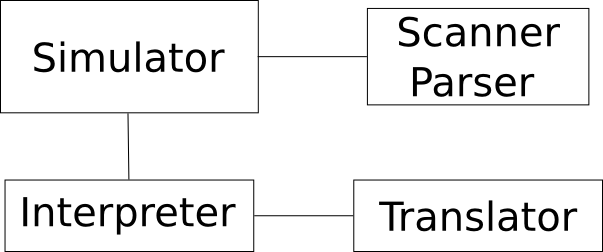
\includegraphics[scale=.6]{block.png}
\end{center}
\end{figure}

The cmulog interpreter consists of several major blocks: scanner,
parser, translator and interpreter. The relationship between these
components is demonstrated in figure *.  The simulator loads each
program by reading in each necessary ``.ul'' file through the scanner
and parser, resulting in an AST.  The each AST is then passed into the
interpreter, resulting in a database of rules and facts in the
interpreter's internal format.  The interpreter does not operator
directly out of the AST, however: it uses the translator to convert
the AST to a ``translated synatax tree'' (TST) first.  

While the AST directly represents the structure of a C$\mu$LOG, there
are a number of static transformations which do not change the meaning
of the program, but make interpreting it much easier for the
interpreter.  The TST represents a simplier version of the program.
The translator removes all the variable names and indexes them to a
list and then each of them are identified by the number rather than
the name.  It also partitions all the statements with and without
side-effects and runs all the ones without side-effects once for each
solution. It performs all possible arithmetic to reduce each statement
into its simplest form. It brings the unknown variable to the leftmost
side by making all the necessary changes. For $(3+4>\$x-1$) will
reduce to ($\$x<6$). Lastly, all the static semantic checking is also
done in the translator.

Using the database reference returned from the interpreter to the
simulator, the simulator (or any other program for that matter) can
query the database using the interpreter's ``query'' method, passing
in the name to query, and the number of parameters.  From this query
method, the solution solver lazily evaluates the query by returning
either ``NoSolution'' or ``Solution''.  ``NoSolution'' indicates the
all the results have already been returned.  ``Solution'' is composed
of a list of constraints (one per parameter) and a function to
generate the next solution.  Each solution is computed when the next
function is called, so if there are an infinite number of solutions,
the query function will not block forever.  The caller may iterate
through all of the solutions, or use only the first one.

Finally, the simulator uses the interpreter to query various terms for
each turn, modifying its state and printing the output.  For instance,
it queries ``wall'' with two parameters (for each coordinate) each
turn, iterates through all of the solutions, and puts a wall at each
solution.  For each agent, it queries the ``move'' term and uses only
the first solution to move each agent.  Before the first move, the
simulator even queries the environment for the ``agent'' term to get
the location of the agent program and its symbol!

Other programs such as the stand-alone ``culog.ml'' interpreter use
the same interpreter interface to parse programs into databases and
query these programs using different terms to invoke different
behaviors.  The stand-alone interpreter queries and ``main'' term and
iterates through the results, and is generally used for testing of the
interpreter.  Other programs could use their own terms to generate
different behaviors.

\section{Test Plan}

\subsection{Testing Script}
The python script shown in listing \ref{testpy} is used to run our
tests.  Each test can be one of three different types: a parsing test,
an interpreter test, or a full simulation test.

\singlespace
\lstset{caption=Testing Script,label=testpy}
\lstinputlisting{../src/test.py}
\onehalfspace 

\subsection{Test Case Rationale}
Most of our test cases are written to test a specific feature.  For
instance, ``andTest.ul'' is designed to test AND blocks.  To whatever
extent possible, these tests avoid testing other features.  This makes
it easier to determine what feature has been broken when tests start
failing.  Other tests are designed to fail to make sure that various
parts of the system fail properly.  Still other tests are composite
tests and are designed to test the system as a whole- they test
multiple features at once to ensure that there are not bizarre
interactions between various parts of the system.

\subsection{Testing Results}
As of the writing of this report, the testing results are shown
below.  Each of the test inputs and outputs can be found in the test
cases appendix.

\begin{verbatim}
Running tests/andTest.ul                   ...OK
Running tests/facts.ul                     ...OK
Running tests/learnForget1.ul              ...OK
Running tests/main.ul                      ...OK
Running tests/main_fall_through.ul         ...OK
Running tests/mult-main.ul                 ...OK
Running tests/neq.ul                       ...FAIL!
Running tests/not1.ul                      ...OK
Running tests/plist-twice.ul               ...OK
Running tests/printer_test.ul              ...OK
Running tests/prsimple.ul                  ...OK
Running tests/prstrings.ul                 ...OK
Running tests/range.ul                     ...OK
Running tests/sim_dot1.ul                  ...OK
Running tests/sim_dot2.ul                  ...OK
Running tests/sim_my_loc.ul                ...OK
Running tests/sim_ndot2.ul                 ...OK
Running tests/sim_two_test.ul              ...OK
Running tests/simulator_test.ul            ...OK
Running tests/sprint1.ul                   ...OK
\end{verbatim}


\section{Lessons Learned}

\subsection{From Devesh}
Programming languages and translators project introduced me to a whole
new world of programming both logic and functional. In the first
project meeting we envisioned a programming language to simulate agent
movement in a grid based environment. The most obvious choice was
having a logic level programming language. The learning course started
with choosing a convinient and accurate grammar. After that working on
the parser and scanner made me realize the power of type checking in
ocaml. I also learnt how to logically reason and resolve the shift
reduce and reduce reduce conflicts. 

Implementation of the interpreter introduced me the power of recursive
programming. Writing tests help me find bugs in the language, also it
taught me that the testing is an ongoing process. Working in a team
and meeting self made deadlines was also part of my learning. 

After the working on this project I found it much easier to understand
the syntax and program in "Murphy" a formal verification
language. Along with programming languages it also exposed me to shell
scripts, Makefiles, Svn repositories.

\subsection{From Nishant}

Programming Languages and Translators, is my first ever core CS
course. Being an EE student it was difficult but seemed interesting
enough a course to be taken. The motivation behind taking this course
was to learn about programming languages and the working of a
translator and the various components a language
interpreter/translator/compiler is made of. Another reason was to get
involved in a programming project to get a feel of programming and
think as a system programmer, designing stuff for the end user.

After taking the class and brain storming with the group members, the
thought was to create this language and looked unsurmountable to
me. As a niche programmer I learnt a few valuable lessons in regards
of thinking as a system programmer. This class and the project has
introduced me to many different types of langauges, like Prolog
(logical) and obviously OCaml(functional). Learning how to program in
OCaml took some doing. Handling the return types and recursion was not
easy. But after a full course and the project it is possible to write
in OCaml.  Adapting to a new language, was a very useful thing learnt
as well. While using a system modelling language called Promela for
another class, I found it extremely easy to adapt to it. The other
most important thing I learnt was errors, their types and their
origin. To conclude, this project has taught me the tricks of the
trade to ``program'' and given me the tool, ``OCaml''.

\subsection{From Cheng}
From this project, I have learned not only how to contruct an
interpreter step by step but also how to collaborate with my
teammates.

Basically, there are three most important things i have learned from
this project. First, I have acquired a deep understanding of basic
concepts covered in the class. This is definitely helpful when I am
trying to study a new programming language. Specifically, I can
quickly learn how to program using this language and solve the
compiling errors as soon as I know about the general features of its
compiler (such as naming and scoping rules). Moreover, the success of
the project is largely determined by its design. With a good design,
coding part will be more easily. However, with a bad design, it will
be a painful experience. So it is wise to spend most time on the
software design. Finally, teamwork plays a key role in software
development. In this project, I have improved my skills of
communication. With better communication, the whole team can work more
efficiently.


\subsection{From John}

A few rules to live by:
\begin{description}
  \item[Tools] Don't use the wrong tools for the right job or the
    right tools for the wrong job.  Even parity is required!  The
    interpreter is written to lazily evaluate queries both to reduce
    memory usage and avoid infinite loops in cases of infinite
    solutions.  This lazy evaluation stragety would have been much
    easier to implement either with co-routines or lazy evaluation (a
    la Haskell.)  Since OCaml offers neither of these features, I
    implemented lazy evaluation by hand, and it made everything harder
    by an order of magnitude.  Since I didn't have the proper tools
    available, I shouldn't have written lazy evaluation.  I should
    have created a logic solver would could only operate on a smaller
    class of programs, and would return all the results at once.

  \item[Testing] Everyong tests while they write code.  You have to.
    Frequently, you write tests in a temporary file and discard when
    the feature is ``working.''  Don't do this.  It's almost always
    worth the extra time to set up a test bed and put your tests in
    it.  Then keep them.  Run them often.  Passing tests gives you a
    warm, fuzzy feeling which grows with the number of tests.  So,
    keep all your ``temporary'' tests and you'll not only feel better
    about yourself, but you'll be ensuring long-term quality.

  \item[Refactoring] At first, you don't know the features of the
    library and language.  You'll write an AST with unnecessary boxing
    and unboxing.  You'll re-write List.filter, and use lambdas when
    currying would have done the job.  Realizing it later on is the
    mark of a good programmer.  Refactoring this code is the mark of a
    diligent one.

  \item[BYOT] Bring your own tools!  Tools are what separate the chaff
    from the wheat.  If you need something done and a tool can do the
    job, write the tool.  Scripting languages are great for this, so
    one of the best time savers is intimate knowledge of a scripting
    language.  Any language will do, but you can't be afraid of using
    it.  Python is my pocket knife of choice, and as far as I'm
    concerned, there's no such thing as abuse!

  \item[Recycling] Does the code you're writing right now look at lot
    like some of the code you wrote yesterday?  Don't write it again,
    refactor the old code into a more generic function.  I won't claim
    to be an angel, but I'm sure that ``copy and paste'' are tools of
    the devil.
\end{description}


\singlespace

\appendix
\section{Appendix: Test Cases}
\include{tests}

\section{Appendix: Code Listings}

\subsection{parser.mly}
\lstset{caption=C$\mu$LOG Parser,label=parser}
\lstinputlisting{../src/parser.mly}

\subsection{scanner.mll}
\lstset{caption=C$\mu$LOG Scanner,label=scanner}
\lstinputlisting{../src/scanner.mll}

\subsection{ast.mli}
\lstset{language=Caml,caption=C$\mu$LOG AST,label=ast}
\lstinputlisting{../src/ast.mli}

\subsection{printer.ml}
\lstset{language=Caml,caption=C$\mu$LOG AST Printer,label=printer}
\lstinputlisting{../src/printer.ml}

\subsection{tst.mli}
\lstset{language=Caml,caption=C$\mu$LOG Translated Syntax Tree,label=tst}
\lstinputlisting{../src/tst.mli}

\subsection{trans.ml}
\lstset{language=Caml,caption=C$\mu$LOG AST to TST Translator,label=trans}
\lstinputlisting{../src/trans.ml}

\subsection{culog.ml}
\lstset{language=Caml,caption=C$\mu$LOG ``General Purpose'' Interpreter,label=culog}
\lstinputlisting{../src/culog.ml}

\subsection{simulator.ml}
\lstset{language=Caml,caption=C$\mu$LOG Simulator,label=simulator}
\lstinputlisting{../src/simulator.ml}

\subsection{interp.ml}
\lstset{language=Caml,caption=C$\mu$LOG Interpreter,label=interp}
\lstinputlisting{../src/interp.ml}

\end{document}
